

\chapter{Estimating the parameters of selective sweeps from patterns of genetic diversity in the house mouse genome}

\chaptermark{Estimating sweep parameters}

\externaldocument{\dir/chapter4Appendix/chapter4appendix.tex}


%%%%%%%%%%%%%%%%%%%%%%%%%%%%%%%%%%%%%%%%%%%%%%%%%%%%
%
%  #   #    #  #####  #####  ######
%  #   ##   #    #    #   #  #    #     
%  #   # #  #    #    #####  #    #
%  #   #  # #    #    #  #   #    #           
%  #   #   ##    #    #   #  #    #  
%  #   #    #    #    #   #  ######    
%
%%%%%%%%%%%%%%%%%%%%%%%%%%%%%%%%%%%%%%%%%%%%%%%%%%%%


\section{Introduction}

	Genetically linked sites do not evolve independently, so that selection acting at one site may influence variation at another one. The consequences of for variation at linked sites are related to the frequency and strength of selected mutations as well as, crucially, the rate of recombination \citep{RN124,RN206,RN287,RN157}. Several modes of selection at linked sites have been identified: selective sweeps (SSWs), caused by the spread of advantageous mutations and background selection (BGS), caused by the removal of deleterious variants, associative overdominance, the effects of balancing selection on linked neutral variability and the effects of local selective differences on between-population neutral divergence.	 Of relevance for this study are SSWs and BGS. Both processes can potentially explain the positive correlations between nucleotide diversity and recombination rate reported in many species \citep{RN117}. However, the proportion of nonsynonymous substitutions attributable to adaptive evolution ($\alpha$) is typically high (50\%) (\citealt{RN215}; but see \citealt{RN352} for caveats), suggesting that SSWs may play a substantial role in shaping nucleotide diversity across the genomes of many species.

	SSWs have been the focus of intense population genetic research \citep{RN124, RN226, RN278, RN235}. The classic footprint of a selective sweep is a trough in nucleotide diversity at neutral sites surrounding substitutions. The reduction in nucleotide diversity caused by a SSW is related to the strength of selection acting on advantageous mutations as well as the frequency with which they arise. Taking advantage of this, \cite{RN277} used a model of SSWs to estimate the frequency and strength of advantageous mutations in \textit{Drosophila melanogaster} by fitting the relationship between recombination rate and nucleotide diversity data for a number of genomic loci. At the time of their analysis, the theory of BGS was in its infancy and models combining the effects of BGS and sweeps had not been developed. However, the effects of BGS are expected to be ubiquitous across the genome \citep{RN116, RN274, RN120}, and studies, conceptually similar to Wiehe and Stephan's (1993), have shown that controlling for BGS is important when parametrizing sweep models from patterns of nucleotide diversity \citep{RN290, RN274, RN116}.

	Both SSWs and BGS reduce nucleotide diversity, so it has proven difficult to distinguish their effects using population genetic data \citep{RN339}. A number of different approaches have been taken to tease apart the effects of the two processes. \cite{RN167} showed that there is a trough in average diversity around recent nonsynonymous protein-coding substitutions in \textit{Drosophila melanogaster}, but not around synonymous ones. Since this pattern is strongly suggestive of SSWs, \cite{RN167} fitted a sweep model to the observed trough and estimated that strongly advantageous mutations ($2N_es$ $\approx$ 5,000) occur in the fruitfly's genome.  In the house mouse, there is also a trough in diversity around recent nonsynonymous substitutions, but there is an almost identical trough around synonymous substitutions, and furthermore a similar trough is observed around  randomly selected synonymous and nonsynonymous sites \citep{RN122}. The overall pattern suggests that the reductions in diversity caused by selection at linked sites extend beyond the average distance separating nonsynonymous substitutions, so that the methods employed by \cite{RN167} are not effective in mice \citep{RN122}. However, values of $\alpha \geq 0.19$ have been reported for  multiple classes of functional elements \citep{RN122} and BGS alone cannot fully explain the observed patterns of diversity (\citealt{RN122}, Chapter 3), suggesting that SSWs contribute to the patterns in mice.


\linespread{1}
\begin{figure}[h!]
   \centering      
   \noindent\makebox[\textwidth]{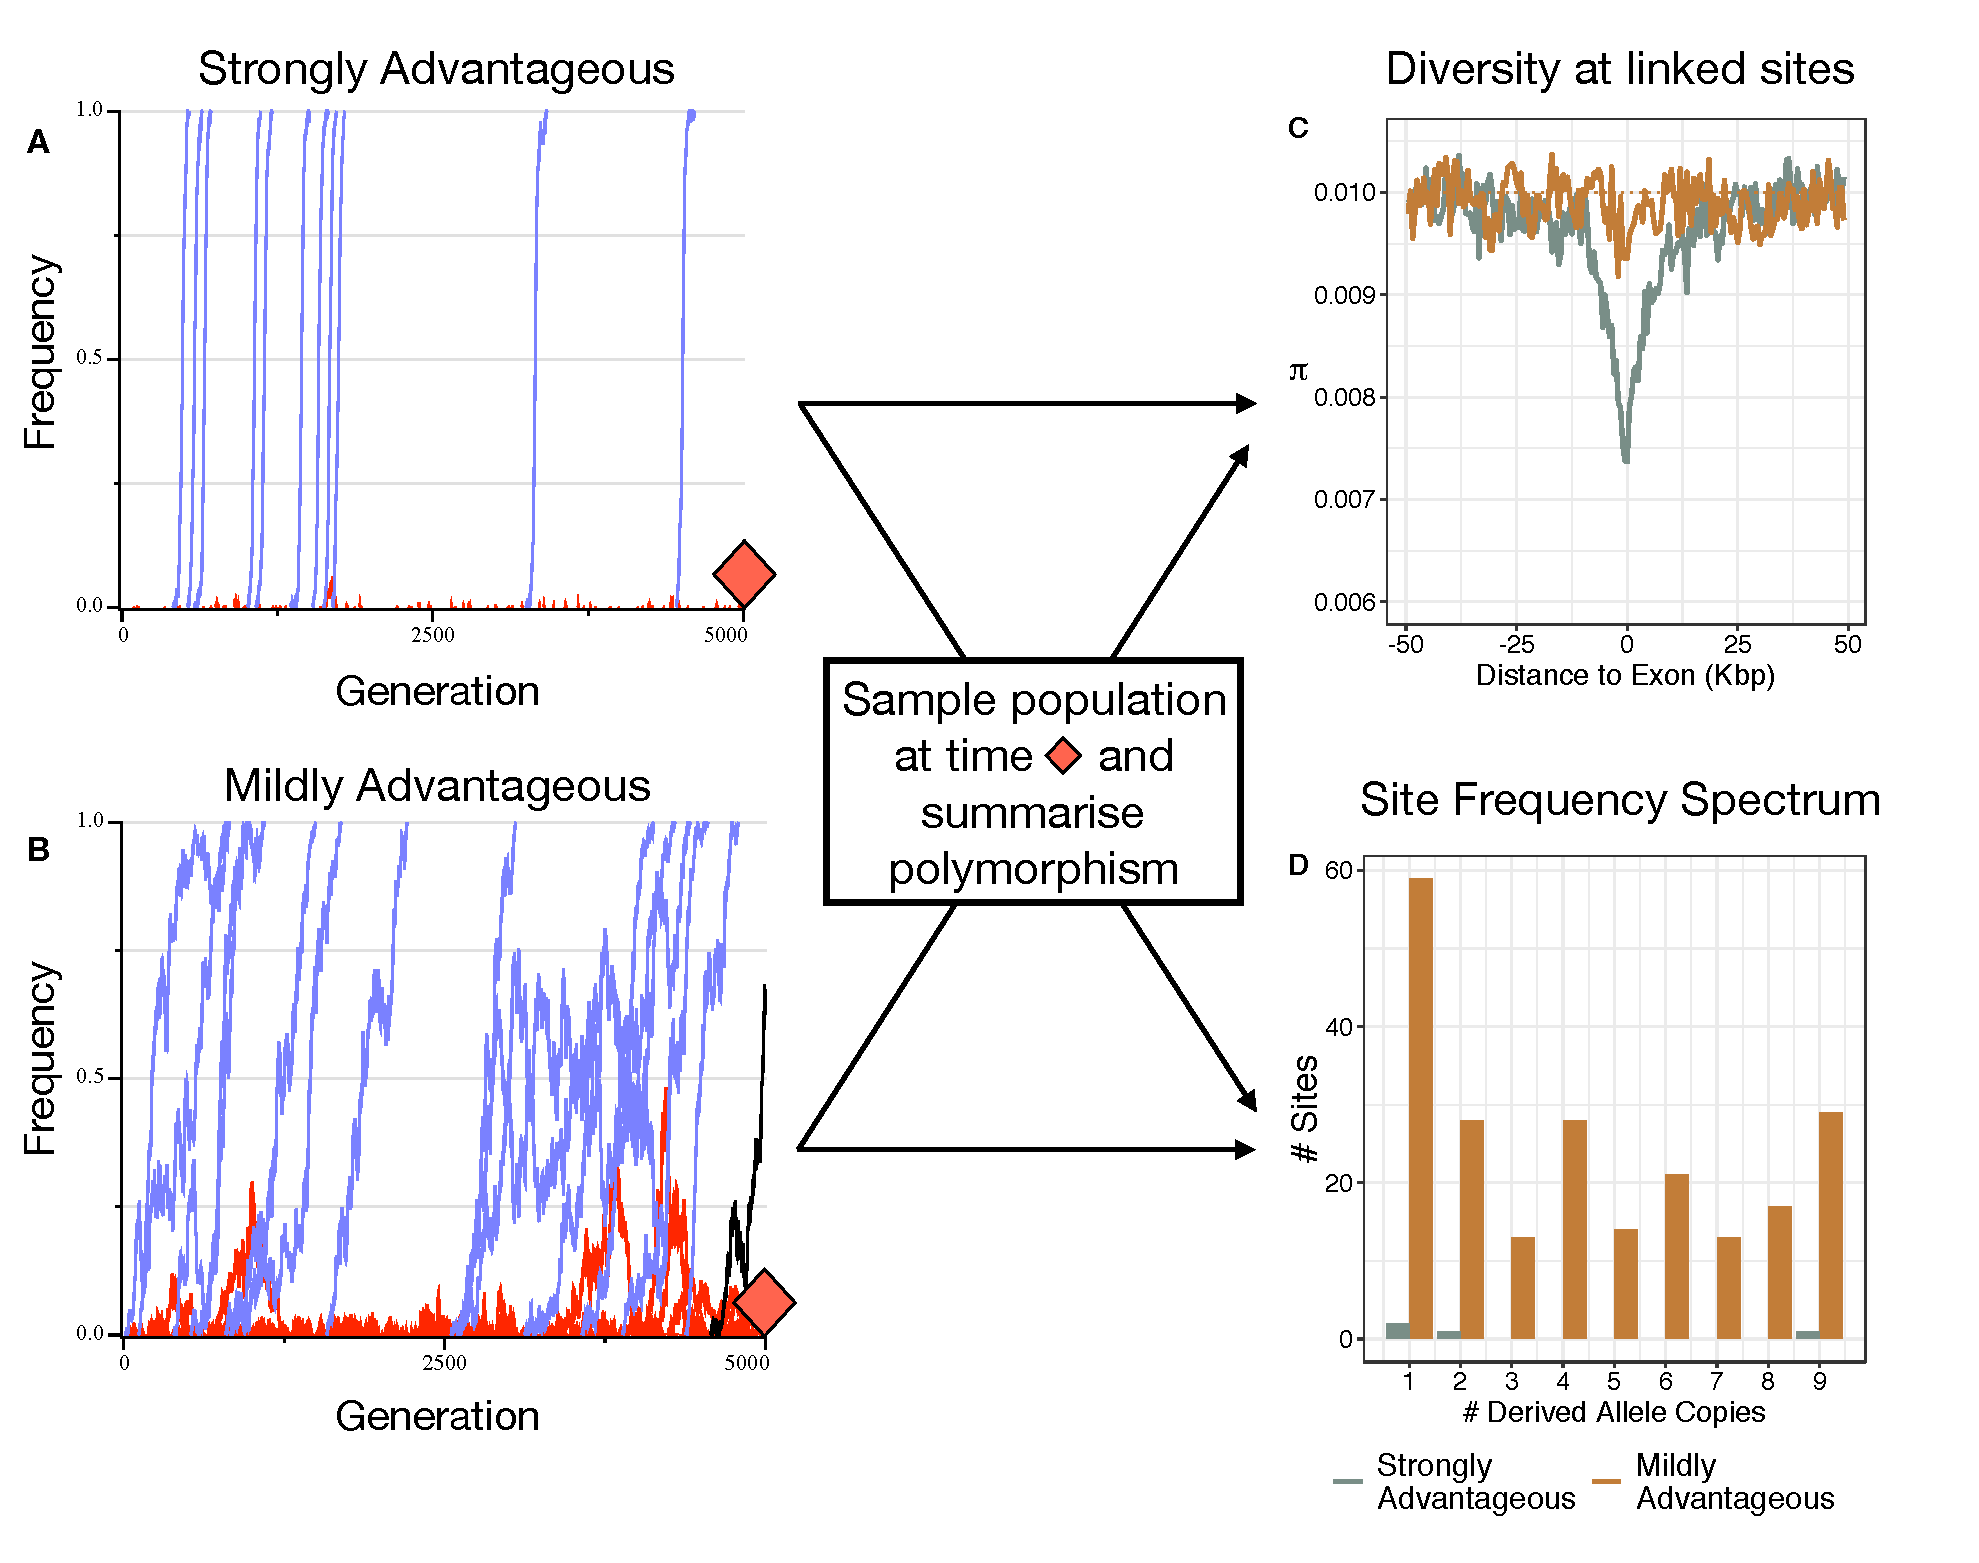
\includegraphics[width=\textwidth]{\dir/chapter4/figures/Trajectories.pdf}}
   
 \caption{A cartoon demonstrating the effect of strongly and mildly advantageous mutations on different aspects of population genomic data. A and B show frequency trajectories for advantageous mutations occurring in a simulated protein-coding exon. The case of infrequent, strongly selected advantageous mutations ($\gamma_a = 400$ and $p_a = 0.00025$) is shown in A. The case of frequent, mildly beneficial mutations ($\gamma_a = 10$ and $p_a = 0.01$) is shown in B. Note that the compound parameter $\gamma_a p_a$, which is directly proportional to the rate of selective sweeps, is the same for the two scenarios. In A and B blue lines represent mutations that went to fixation, red lines are mutations that were lost through drift and black lines are mutations that were polymorphic at the end of the simulation. Panel C shows the reduction in neutral diversity in regions surrounding a 1,000bp exonic region. D shows the site frequency spectra for advantageous mutations. Simulations were performed using the SLiMgui available at https://messerlab.org/slim/.}.
 
 \label{fig:Cartoon}
\end{figure}
\linespread{2}

	In Chapter 3, we sought to tease apart the contributions of BGS and SSWs to patterns of diversity in mice. By analysing unfolded site frequency spectra (uSFS), we estimated positive selection parameters, but found that these could not explain the troughs in nucleotide diversity around functional elements in the mouse genome. One explanation for our findings is that infrequent, strongly advantageous mutations, which may substantially influence diversity at linked sites, will make little contribution to standing variation and are thus undetectable by analysis of the uSFS \citep{RN290}. Figure \ref{fig:Cartoon} demonstrates how, for a given rate of sweeps, frequent mildly or infrequent strongly selected advantageous mutations may influence different aspects of population genomic data. The frequency trajectories in Figure \ref{fig:Cartoon} clearly show how weakly selected mutations take longer to fix and contribute more to standing variation than do strongly selected mutations. Furthermore, Figure \ref{fig:Cartoon} shows how strongly selected mutations in the population result in a marked reduction in diversity around the simulated exon, while contributing very little to standing variation (i.e. the uSFS). On the other hand, mildly advantageous mutations do not substantially affect linked diversity, but do contribute substantially to standing variation. Although only a cartoon, Figure \ref{fig:Cartoon} shows how, depending on the underlying parameters, different summaries of population genomic data are more or less informative for inferring positive selection. The methods we used in Chapter 3 relied on the assumption that selected mutations segregate in populations of interest, such that they affect the shape of the uSFS. Since the parameter estimates we obtained from the uSFS cannot explain the dips in diversity in mice, a more powerful approach for inferring the strength of positive selection may be to apply a model of selective sweeps to the observed data.
	
	In this study, we use a model of SSWs to estimate the strength and frequency of advantageous mutations in protein-coding exons and regulatory elements. Specifically, we find that the strength of selection acting on protein-coding exons is far greater than that acting on regulatory elements. Using simulations, we demonstrate that the inferred parameters of positive selection are likely out of the range detectable by analysis of the uSFS.  Finally, using a simple model of the fitness change brought about by adaptive evolution, we show that, despite adaptation occurring more frequently in regulatory regions, adaptation in protein-coding regions may contribute more to phenotypic evolution in mice.


%%%%%%%%%%%%%%%%%%%%%%%%%%%%%%%%%%%%%%%%%%%%%%%%%%%%
%
% #   #  ####  #####  #   #  ####    ####
% ## ##  #       #    #   #  #   #   #  
% # # #  ###     #    #####  #   #   ####
% #   #  #       #    #   #  #   #      #        
% #   #  #       #    #   #  #   #      #
% #   #  ####    #    #   #  ####    ####
%
%%%%%%%%%%%%%%%%%%%%%%%%%%%%%%%%%%%%%%%%%%%%%%%%%%%%
\section{Materials and Methods}

\subsection{Model of selective sweeps with background selection}

	\cite{RN290} gave expressions for the neutral diversity expected under the combined effects of BGS and SSWs. The model of sweeps they assumed considers the case of a haplotype carrying a neutral mutation at site $k$. A new semi-dominant advantageous mutation with selection coefficient $s_a$ occurs at site $i$ on the haplotype and spreads to fixation, affecting a change in the frequency of the neutral allele. Recombination between sites $i$ and $k$ uncouples the neutral and selected alleles at rate $r_{i,k}$. The change in neutral diversity at site $k$ ($\Delta \pi_k$), relative to its expectation in the absence of selection ($\pi_0$) is given by
	
\begin{equation}
\label{piChange}
\frac{\Delta \pi_{k}}{\pi_{0}} \approx -(2N_e s_a)^{\frac{-4r_{i,k}}{s_a}} .
\end{equation}
	
	\noindent
Where $N_e$ is the effective population size. This approximation assumes that selection on the advantageous allele satisfies $N_es_a > 1$ such that the sweep can be treated deterministically following its escape from drift. See \cite{RN235}, \cite{RN173}, or \cite{RN290} for a full derivation of Equation \ref{piChange}. 
		
	Equation \ref{piChange} can be thought of as the probability that a neutral allele is caught in the sweep, or as the probability of sweep-induced coalescence. For a particular class of functional elements (e.g. protein-coding exons), sweeps occur at a rate of $V_{a} = 2 \mu p_{a} \gamma_{a}$  per nucleotide per generation (Kimura and Ohta 1971), where $\mu$ is the point mutation rate per nucleotide, $p_a$ is the proportion of new mutations that are advantageous and $\gamma_a$ is the scaled selection coefficient ($2N_es_a$) of those mutations. If $V_a$ is sufficiently low, such that one sweep does not interfere with another, the total probability of sweep-induced coalescence for a neutral site caused by selection at a linked functional element is
	
\begin{equation}
\label{singleClass}
P_{sc,k} \approx V_a \tau\gamma_a^{\frac{-4r_{i,k}}{s_a}}.
\end{equation}

\noindent
Where $\tau$ is the average number of sites in a particular class of functional elements. This model assumes that $N_e$ has remained constant for the timescale of the effects of sweeps and that there is full recovery of diversity between sweeps When assuming that recombination proceeds solely by crossing over, $r_{i,k}$ is simply the product of the physical distance ($d_{i,k}$) and the local crossing-over rate ($r_c$). When incorporating gene conversion, we use Equation 1 from \cite{RN379}:
 
\begin{equation}
\label{geneConversion}
r_{i,k} = d_{i,k} r_c + 2 g_c d_g \Bigg( 1 - e ^{-\frac{d_{i,k}}{d_g}} \Bigg)
\end{equation} 
\noindent 
where $g_c$ is the rate of gene conversion and $d_g$ is the mean gene conversion tract length, assuming that the distribution of tract lengths is exponential. When applying Equation \ref{geneConversion} we use $g_c = \kappa r_c$ where $\kappa$ is the ratio of the non-crossovers to crossovers.
	

	The effects of BGS can be thought of as a reduction in the effective population size at a neutral locus by some fraction $B_k$. The probability of coalescence for a neutral allele affected by BGS is thus $\frac{1}{B_k 2N_e}$. If it is assumed that BGS and SSWs are independent exponential processes, the rate of coalescence induced by the two is simply the sum of $\frac{1}{2N_e B_k}$ and $P_{sc,k}$. We scale the sweep effect $P_{sc,k}$ by $B_k$ to reflect the reduction in the fixation probability for a new advantageous mutation given the reduced $N_e$ under BGS \citep{RN349}. Taking the reciprocal of the rate of coalescence at the neutral site given the combined effects of BGS and SSWs ($T_k$) and expressing it relative to the expected rate of coalescence under neutrality ($T_0$) gives

\begin{equation}
\label{jointApprox}
\frac{T_k}{T_0} \approx \frac{\pi_{k}}{\pi_{0}} \approx  \frac{1}{B_{k}^{-1}  + 2N_eB_{k}P_{sc,k}}.
\end{equation}
\noindent
	Where $\pi_k$ is genetic diversity observed at neutral site \textit{k} and $\pi_0$ is diversity expected in the absence of selection at linked sites. 
	
	Both theoretical and experimental results suggest that the distribution of fitness effects for advantageous mutations is exponential \citep{RN109}. We incorporate an exponential distribution of advantageous mutational effects in Equation 3 as follows:

		\begin{equation}
		\label{exponential}
P_{sc,k} \approx \int \limits_{0}^{\infty} f(\gamma_a) V_a \tau\gamma_a^{\frac{-4r_{i,k}}{s_a}} \mathop{d\gamma_a}.
		\end{equation}

	We estimated $\gamma_a$ and $p_a$ by fitting Equation \ref{jointApprox} to the relationship between nucleotide diversity and genetic distance to functional elements using non-linear least squares with the \emph{lmfit} (0.9.7) package for Python 2.7. When analysing the mouse data (see below) we compared the fit of Equation \ref{jointApprox} incorporating either one or two discrete classes of advantageous mutations (Equation \ref{singleClass}) or the exponential distribution (Equation \ref{exponential}) using Akaike's Information Criterion (AIC). In the context of nonlinear least squares, the quantity being minimised is the sum of squares about the curve. Under a given model, if a normal distribution of residuals about the curve estimated by least squares is assumed, then the AIC can be calculated from the maximum likelihood estimated of the residual variance (pg60-64 of Burnham and Anderson 2002). Standard errors in nonlinear least squares are derived from the covariance matrix of the best-fitting parameters.
		
	\subsection{Analysis of mouse data}

	We analysed patterns of genetic diversity in 10 wild-caught \textit{M. m. castaneus} individuals, first reported by \cite{RN122}. Briefly, \cite{RN122} sequenced individual genomes to high coverage ($\approx$ 30x) using Illumina paired-end reads, which were then mapped to the mm9 mouse reference genome using BWA \citep{RN251}. Variants were called using a Samtools pipeline \citep{RN252}. Note that we only analyse SNP data in this study, and insertion/deletion variants are not included. For further details of the sequencing and variant calling methods, see \cite{RN122}. Protein-coding exons annotated in version 67 of the Ensembl annotation database, and the locations of conserved non-coding elements (CNEs) identified by \cite{RN122} using an alignment of placental mammals, were used in this study. The mean length of a protein-coding exon is 151bp, of which we assume 75\% are subject to selection. The mean length of a conserved non-coding element is 51bp, of which 100\% of sites are assumed to be subject to selection.

	From the edges of exons (CNEs), polymorphism data and divergence from the rn4 rat reference genome were extracted for non-CpG-prone sites in windows of 1Kbp (100bp) extending to distances of 100Kbp (5Kbp). Non-CpG-prone sites were operationally defined as those that are either preceeded by a C or suceeded by a G in either the 3' to 5' or 5' to 3' directions in the reference genome. Analysis windows were then binned based on genetic distance to the focal element. Genetic distances were calculated using either the linkage disequilibrium (LD) based recombination map for \textit{M. m. castaneus} constructed by \cite{RN340} or the pedigree-based genetic map constructed using common lab strains of \textit{M. musculus} by \cite{RN232}. Because LD-based and pedigree-based recombination maps have different advantages and shortcomings (\textit{see Results}), we performed analyses based on both of these maps in parallel.

	Compared to crossingover rates, gene conversion parameters are very difficult to estimate \citep{RN247}. Empirical estimates of the ratio of crossovers to non-crossovers (a parameter we have termed $\kappa$) vary by orders of magnitude in mammals \citep{RN247}. \cite{RN263} measured non-crossover gene conversion rates in three recombination hotspots in mice and estimated a mean gene conversion tract length of 144bp and $\kappa = 0.105$, we refer to this estimate as the low gene conversion rate. \cite{RN263} pointed out that they likely underestimated the gene conversion rate. Since values of $\kappa$ as high as 12.0 have been reported in humans \citep{RN247}, we explored the effects of high gene conversion rates on the parameters of SSWs inferred from models of selection at linked sites, we also assumed $\kappa$ = 12.0, which we refer to as the high gene conversion rate. 

	In order to disentangle the sweep parameters we obtained by fitting Equation \ref{jointApprox}, we assume a point mutation rate of $5.4 \times 10^{-9}$, which is based on a mutation-accumulation experiment in \textit{M. musculus} \citep{RN228}. We also assume an $N_e$ for \textit{M. m. castaneus} of 426,200, based upon the level at which neutral diversity plateaus in the regions surrounding CNEs.

	\subsection{Estimates of \textit{B}} 
 
 	BGS contributes to the troughs in diversity around both protein-coding exons and CNEs (\citealt{RN122}; Chapter 3). We therefore required estimates of the effect of BGS on neutral diversity, \textit{B}, to use as a covariate when fitting Equation \ref{jointApprox} to diversity troughs. Analytical formulae for calculating \textit{B} over-predict the effects of BGS when purifying selection is weak ($\gamma_d < 1$) \citep{RN380,RN378}, and since weakly deleterious mutations comprise a large portion of the DFEs estimated for mice (\citealt{RN122}, Chapter 3), we opted to obtain \textit{B} from simulations.
 	
 	In Chapter 3, we used simulations to estimate the contribution of BGS to patterns of nucleotide diversity around both protein-coding exons and CNEs. We incorporated the actual distribution of the protein-coding genes (modelling both exons and untranslated regions) as well as CNEs into our simulations. The dDFEs we estimated for the 0-fold sites, untranslated regions and CNEs in Chapter 3 were incorporated into the simulations. Recombination rate variation was included in simulations assuming the \textit{castaneus} map. Simulations of $N = 1000$ diploid individuals were run for 10,000 generations. At the endpoint of simulations, we sampled 200 haploid chromosomes from the population and extracted $B = \frac{\pi}{\pi_0}$ as a function of genetic distance from both protein-coding exons and CNEs. We used these estimates of \textit{B} when fitting Equation \ref{jointApprox}. The simulations described here were identical to those we used in Chapter 3, except that we increased the number of simulation replicates from 2,000 to 6,000. 
 	
 	To obtain smoothed $B$ values we fitted Loess curves to the simulation data using R (v3.4.2), using a span parameter of 0.2 and using the number of sites contributing to each analysis bin as weights. Simulations were performed in SLiM (v1.8; \citealt{RN148}). 

	\subsection{Simulating the unfolded site frequency spectra}
	
	Figure \ref{fig:Cartoon} demonstrates that, for given rate of sweeps, different aspects of population genomic data may be informative for inferring positive selection if advantageous mutations occur frequently, but have mild fitness effects, or are infrequent, but are strongly beneficial. In Chapter 3 of this thesis, we estimated the frequency and strength of selection acting on advantageous mutations in \textit{M. m. castaneus} by analysing the uSFS, but found that the parameter estimates we obtained could not explain troughs in diversity observed around either protein-coding exons or CNEs. A possible explanation for our inability to explain the observed patterns is that the advantageous mutations involved are strongly selected and infrequent, and are thus difficult to estimate by analysis of the uSFS (see Introduction).
		
	We tested the hypothesis that infrequent, strongly advantageous mutations are difficult to detect by analysis of the uSFS using simulations. We generated simulated datasets using the forward-time simulation package SLiM (v1.8; \citealt{RN148}). We simulated the evolution of 1Mbp chromosomes containing 20 evenly spaced  `genes`. Each `gene` consisted of ten 100bp exons, separated by 1Kbp of neutrally evolving intronic sequence. We modelled nonsynonymous mutations as 75\% of mutations occurring in exons, and the remaining 25\% were strictly neutral (i.e. synonymous sites). We varied the $\gamma_a$ and $p_a$ parameters across simulations, but kept the product $\gamma_a p_a$ equal to 0.1. We based this value of $\gamma_a p_a \approx 0.1$ on a recent study of\textit{D. melanogaster} \citep{RN321}. All simulations incorporated the same gamma dDFE (shape parameter $\beta$ = 0.2 and mean $\hat{\gamma_d}$ = -1,000), but the advantageous mutation parameters varied, and are listed in Table \ref{tab:polyDFE} in the Results section. The population-scaled mutation and recombination rates (i.e. $\theta$ = \emph{$4N_{e}\mu$} and $\rho$ = \emph{$4N_{e}r$}, respectively) were set to 0.01. Populations of $N$ = 1,000 diploid individuals were simulated for an initial burn-in of 10$N$ generations to establish equilibrium conditions. After the burn-in, 20 haploid chromosomes were sampled every 2$N$ generations for a further 100$N$ generations. We performed 10 replicate simulations for each set of selection parameters. Across simulation replicates, time-points and loci we extracted simulated nonsynonymous and synonymous sites, giving uSFS data for 10,000 `genes'. We sampled the set of 10,000 `genes' with replacement 100 times, collating the nonsynonymous and synonymous site uSFSs for each replicate.
	
	We estimated our simulated DFEs by analysis of the uSFS using the methods of \cite{RN354}, as implemented in the polyDFE (v1.1) package. polyDFE fits an expression for the uSFS expected in the presence of both advantageous and deleterious mutations to data from putatively neutral and selected classes of sites, and estimates parameters by maximum likelihood. The neutral class is used to determine distortions to the uSFS caused by processes such as selection at linked sites and a history of population size change. In addition, polyDFE corrects for polymorphism misattributed to divergence, mutation rate variability and error in assigning sites as ancestral/derived. \cite{RN354} performed extensive simulations and showed that accurate estimates of the parameters for both deleterious and advantageous mutations can be obtained using their methods. However, there are a range of parameters that they did not test which may be biologically relevant, specifically when advantageous mutations are strongly selected, but infrequent.

	 We analysed the simulated uSFS data using polyDFE choosing Model C (a gamma dDFE and a discrete class of advantageous mutations) and either including or not including between-species divergence. We analysed the uSFS for simulated nonsynonymous sites using synonymous sites as the neutral reference class. For each of the advantageous mutation parameter sets tested, we analysed 100 bootstrap samples of the simulation data.
 
 	
%%%%%%%%%%%%%%%%%%%%%%%%%%%%%%%%%%%%%%%%%%%%%%%%%%%%
%
% ####   ####  #####  #   #  #     #######  #####
% #   #  #     #      #   #  #        #     #
% ## #   ###   #####  #   #  #        #     #####
% # #    #         #  #   #  #        #         #
% #  #   #         #  #   #  #        #         #
% #   #  ####  #####  #####  #####    #     #####
%
%%%%%%%%%%%%%%%%%%%%%%%%%%%%%%%%%%%%%%%%%%%%%%%%%%%%


\section{Results}

\subsection{Patterns of genetic diversity around protein-coding exons and conserved non-coding elements}


	In this study, we analysed the relationship between nucleotide diversity and genetic distance from functional elements in \textit{M. m. castaneus} assuming either a high resolution recombination map constructed using LD (Chapter 2; \citealt{RN340}) (the \textit{castaneus} map) or a pedigree-based map \citep{RN232} (the Cox map). The two methods for constructing recombination rate maps have advantageous and disadvantages. For example, the population-scaled recombination rate ($\rho$) can be inferred from a relatively small sample of unrelated individuals at very fine-scales using LD. However, selection at linked sites influences local LD and may therefore affect recombination rate estimates obtained in this way \citep{RN370}. Alternatively, direct estimates of the recombination rate ($r$) can be obtained from crossing experiments, but to achieve a high resolution recombination map a very large number of individuals need to be genotyped, and this has typically precluded the use of whole-genome re-sequencing, thereby limiting resolution. When analysing patterns of genetic diversity under a model of selection at linked sites, the way in which recombination rate estimates were obtained may, therefore, affect parameter estimates.

	Polymorphism data were extracted from genomic windows surrounding protein-coding exons and CNEs, genetic distances to focal elements were calculated assuming either an LD-based or a pedigree-based recombination map. The choice of recombination map used had a substantial effect on patterns of nucleotide diversity around both protein-coding exons and CNEs (Figure \ref{fig:Diversity2x2}). In the immediate flanks of both exons and CNEs, we found that diversity was lower when assuming the LD-based \textit{castaneus} map than when assuming the pedigree-based Cox map (Figure \ref{fig:Diversity2x2}). Additionally, genetic diversity plateaued at higher levels (Figure \ref{fig:Diversity2x2}). These differences are consistent with the possibility that the Cox map, which was constructed with a far smaller number of markers than the \textit{castaneus} map, does not fully capture regions with both low and high recombination rates. A consequence of this would be, for example, that analysis windows tightly linked to functional elements appear less tightly linked. The choice of recombination map will, therefore, have an impact on the parameters of selection inferred from the patterns of diversity shown in Figure \ref{fig:Diversity2x2}. Throughout the rest of this chapter, we present the results of analyses based on the \textit{castaneus} map together with those based on the Cox map.

\linespread{1}
\begin{figure}[h!]
   \centering      
   \noindent\makebox[\textwidth]{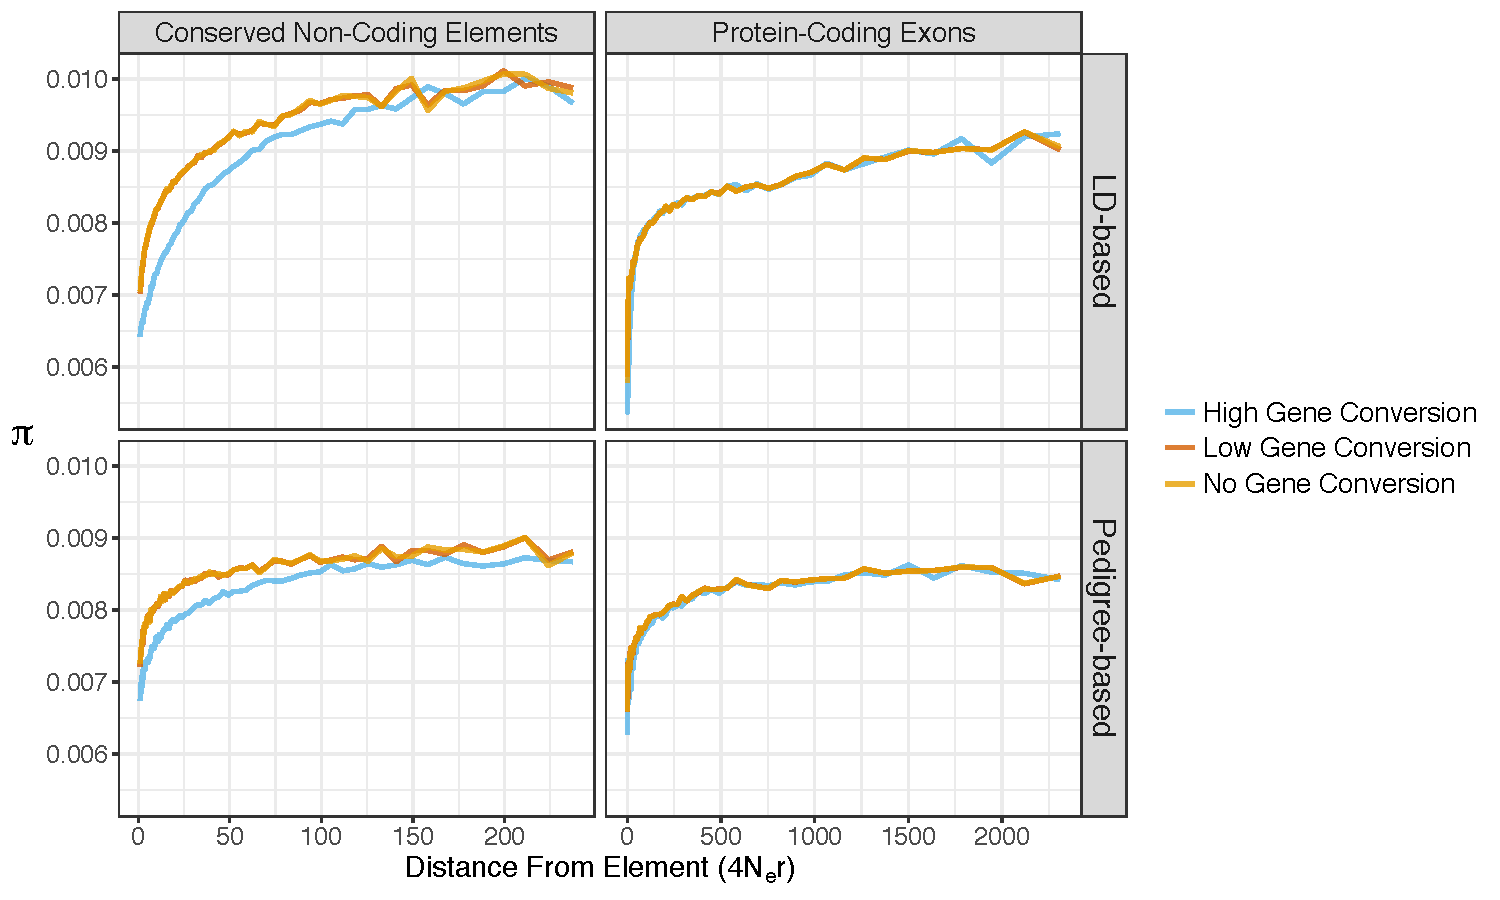
\includegraphics[width=\textwidth]{\dir/chapter4/figures/Pi_geneticDistance_4x4.pdf}}
 \caption{Nucleotide diversity in regions surrounding protein-coding exons and conserved non-coding elements in wild mice, assuming different rates of gene conversion. Population-scaled genetic distances ($4N_er$) were calculated using either an LD-based recombination map constructed for \textit{M. m. castaneus} or a pedigree based genetic map constructed for \textit{M. musculus}. Note that the lines for the cases of no gene conversion and low gene conversion are highly similar.}.
 
 \label{fig:Diversity2x2}
\end{figure}
\linespread{2}

	 Assuming the gene conversion parameters estimated by \cite{RN263} (i.e. a low gene conversion rate) had little effect on the patterns of genetic diversity around both classes of element (Figure \ref{fig:Diversity2x2}). Assuming a higher rate of gene conversion (i.e. 12 times the number of noncrossovers to crossovers) made more of a difference, particularly for CNEs (Figure \ref{fig:Diversity2x2}). The reason for this is that gene conversion will increase the recombination distance between two points proportionally more if analysis windows are physically short than if they are long (Equation \ref{geneConversion} and the reductions in diversity around CNEs are about 10 times narrower than those around exons on a scale of physical distance \citep{RN122}. 
	 	 
\subsection{Diversity expected in the absence of selection, $\pi_0$}

	A key parameter in the model of SSWs and BGS investigated in this study is $\pi_0$, the nucleotide diversity expected in the absence of selection at linked sites. This parameter is very difficult to estimate and may even prove unobservable to be in real data given the ubiquity of selection effects at linked sites \citep{RN357}. One strategy for estimating $\pi_0$ is to divide the mean $\pi$ in regions distant from functional elements by the corresponding value of $B$, the reduction in neutral diversity caused by BGS. $B$ plateaus at approximately 0.95 in regions surrounding both protein-coding exons and CNEs (Figure {\ref{fig:BGSLoess}), but the level at which observed diversity plateaus is different for the two classes of elements (Figure \ref{fig:Diversity2x2}). It may be, then, that the diversity reducing effects of SSWs at elements linked to exons have been greater than for elements linked to CNEs. Because of this difference, and the similarity in BGS effects around the two classes of sites, simply dividing observed $\pi$ by $B$, would give an underestimate of $\pi_0$ as it would not incorporate the reduction in diversity caused by SSWs at linked elements. In addition, the levels at which diversity plateaus in the regions surrounding protein-coding exons and CNEs differ depending on which recombination map is assumed (Figure \ref{fig:Diversity2x2}).	When analysing patterns of diversity around protein-coding exons, we assumed $\pi_0$ values of 0.00955 and 0.00895 when analyses were based on the \textit{castaneus} and Cox maps, respectively. When analysing patterns of diversity around CNEs, we assumed $\pi_0$ values of 0.0102 and 0.00915 when analyses were based on the \textit{castaneus} and Cox maps, respectively.

\subsection{Parameters of selective sweeps obtained from patterns of nucleotide diversity}

	We fitted a model of SSWs and BGS to the reductions in diversity around exons and CNEs, and found that two classes of advantageous mutational effects typically gave a substantially better fit to the data than did a single class or an exponential distribution (as judged by AIC differences; Table \ref{tab:AICcomparison})). This result held regardless of the recombination map assumed and whether or not gene conversion was included. The only exception was that an exponential distribution gave the best fit when protein-coding exons were analysed using the \textit{castaneus} map with the high gene conversion rate, but in this case the AIC differences between the competing models were fairly small (Table \ref{tab:AICcomparison}).
	
\linespread{1}
\begin{table}[H]
   \centering
      \begin{threeparttable}[b]
\caption{Differences in fit for models of advantageous mutations when fitted to troughs in diversity around CNEs or protein-coding exons. Cells with no values indicate the best-fitting models.}


\begin{tabular}{ccccc}
\toprule
	& & & \multicolumn{2}{c}{$\Delta AIC$} \\
       Map & GC & Model\tnote{a} &  CNEs &  Exons \\
\midrule
 \multirow{9}{*}{\textit{castaneus}} &    \multirow{3}{*}{High} &     2 &       &        \\
  &      &     e &   -367 &    -284 \\
  &      &     1 &    -85.6 &    -284 \\ \cdashline{2-5}
  &     \multirow{3}{*}{Low}  &     2 &       &        \\
  &      &     e &   -280 &    -134\\ 
  &      &     1 &   -113 &    -161\\ \cdashline{2-5}
  &     \multirow{3}{*}{None}  &     2 &       &        \\
  &      &     e &   -262 &    -127 \\
  &      &     1 &    -87.3 &    -153 \\ 
\hdashline
\multirow{9}{*}{Cox}  &     \multirow{3}{*}{High} &     2 &       &      -3.91\\
  &      &     e &   -177&        \\
  &      &     1 &    -92&      -1.48\\ \cdashline{2-5}
  &     \multirow{3}{*}{Low} &     2 &       &        \\
  &  	 &     e &   -147 &     -16.2\\
  &      &     1 &    -43.5 &     -32.1\\ \cdashline{2-5}
  &     \multirow{3}{*}{None} &     2 &       &        \\
  &      &     e &   -150&     -19.6\\
  &      &     1 &    -44.0&     -38.9\\ 
\bottomrule
\end{tabular}
 
   \begin{tablenotes}
     \item[a] Denotes the model of advantageous mutations used. $e$ - exponential, $2$ - two classes of discrete effects and $1$ - a single class of discrete effects.
   \end{tablenotes}
  \label{tab:AICcomparison}

  \end{threeparttable}
  
\end{table}
\linespread{2}

	For both protein-coding exons and CNEs we inferred that there is a class of strongly advantageous mutations and a class of more mildly beneficial mutations (Table \ref{tab:EstimatesCastaneus}). When assuming the \textit{castaneus} map and the low gene conversion rate, we estimated the scaled effect of advantageous mutations ($\gamma_a$) was 8,470 and 432 for protein-coding exons and CNEs, respectively. The proportion of new mutations that possess these strongly advantageous selection coefficients were 2.2 x $10^{-5}$ and 1.12 x $10^{-3}$ for protein-coding exons and CNEs, respectively. We also inferred that there is a more mildly beneficial class of advantageous mutations affecting both protein-coding exons and CNEs, which had scaled effects of 22.3 and 14.5, respectively. The proportion of new mutations possessing the more mild selective effects were 0.0202 and 0.0298 for protein-coding exons and CNEs, respectively. With the \textit{castaneus} map, the inferred mildly beneficial mutation parameters were fairly similar to ones obtained by analysis of the uSFS in Chapter 3.

\linespread{1}


\begin{sidewaystable}[H]
\caption{Parameters of positive selection in \textit{M. m. castaneus} estimated by fitting a model of selective sweeps to troughs in diversity around functional elements. The frequency ($p_a$) and scaled selection coefficients ($\gamma_a$) for the two classes of advantageous effects are given. Parameters were obtained assuming background selection and the gene conversion parameters from \cite{RN263}. Standard errors are shown in square brackets below point estimates.}
\centering
	\label{tab:EstimatesCastaneus}
        \begin{tabular}{cccccc}

        \hline
  %            & \multicolumn{2}{c}{} & \multicolumn{2}{c}{}  \\
  Element  &  $\gamma_{a,1}$ & $p_{a,1}$ &$\gamma_{a,2}$ & $p_{a,2}$ &  \\ [0.5ex] \hline

\multirow{2}{*}{Protein-Coding Exons} &  8,470 & 2.22 x $10^{-5}$ & 22.3 & 0.0202 & \multirow{4}{*}{\textit{castaneus} map}\\
   &  [ 672 ] & [ 2.21 x $10^{-6}$ ]& [ 3.39 ] & [ 4.38x $10^{-3}$ ] & \\ 
\multirow{2}{*}{Conserved Non-Coding Elements}  & 432 & 1.12 x $10^{-3}$ & 14.5 & 0.0298 & \\
  &   [ 21.2 ] & [ 8.86 x $10^{-5}$ ]& [ 3.17 ] & [ 8.22 x $10^{-3}$ ] &\\ \hdashline
\multirow{2}{*}{Protein-Coding Exons} &  4,100 & 2.45 x $10^{-5}$ & 117 & 6.16 x $10^{-4}$  & \multirow{4}{*}{\textit{Cox} map}\\
   &  [ 640 ] & [ 5.56 x $10^{-6}$ ]& [ 49.9 ] & [ 2.78 x $10^{-4}$ ] & \\ 
   
\multirow{2}{*}{Conserved Non-Coding Elements}  & 357  &  4.77 x $10^{-4}$ & 5.95 & 0.0454 & \\
  &   [ 46.8 ] & [ 9.37 x $10^{-5}$ ]& [ 3.533 ] & [  0.0358 ] &\\ \hline
        \end{tabular}
   
\end{sidewaystable}


\linespread{2}	
	
	The choice of recombination map strongly affected the estimated selection parameters obtained by fitting patterns of genetic diversity. Use of the pedigree-based Cox map resulted in estimated selection coefficients that were typically smaller than the parameters obtained when assuming the LD-based \textit{castaneus} map (Table \ref{tab:EstimatesCastaneus}). This is presumably because we found the troughs in diversity around both classes of elements to be shallower when calculating genetic distances using the pedigree-based map than when using the LD-based map (Figure \ref{fig:Diversity2x2}).
	
	BGS contributes to the troughs in diversity around both protein-coding exons and CNEs, and causes an overall reduction in neutral diversity (Figure \ref{fig:castaneusFit}). Ignoring the contribution of BGS by setting $B$ to 1.0 when fitting Equation \ref{jointApprox} to the diversity troughs resulted in a much poorer model fit (Table \ref{tab:BGSeffect}). In the absence of BGS effects, the selection coefficents of advantageous mutations required to explain the observed data are far higher (Table \ref{tab:BGSeffect}), consistent with \cite{RN290}. 
	
\linespread{1}
\begin{figure}[h!]
   \centering      
   \noindent\makebox[\textwidth]{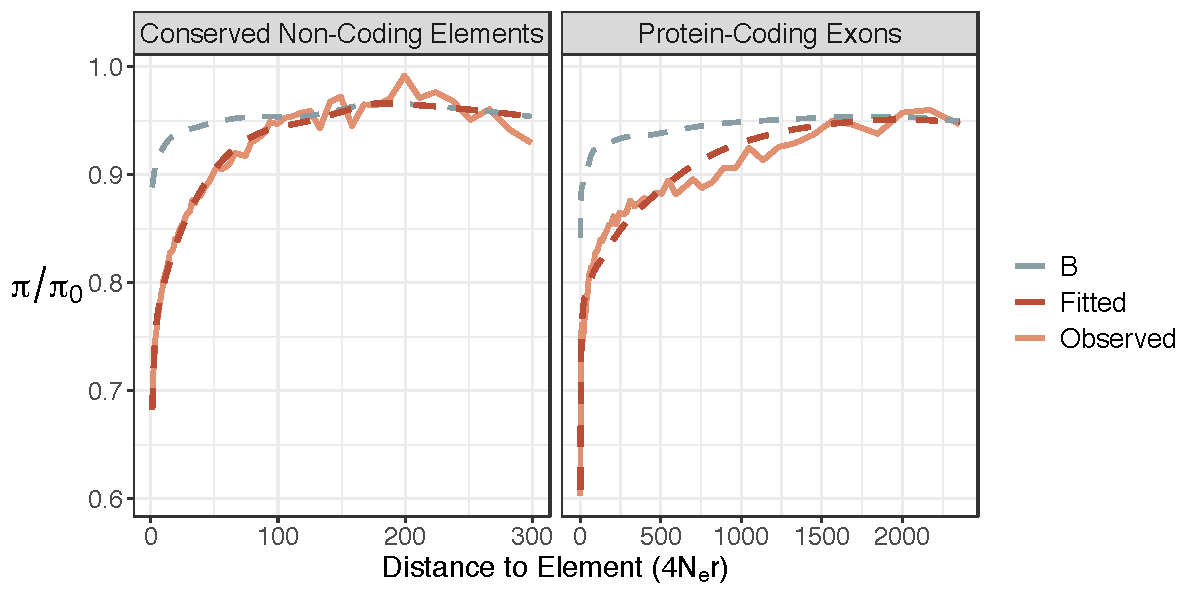
\includegraphics[width=\textwidth]{\dir/chapter4/figures/ModelFit.pdf}}
 \caption{The pattern of scaled nucleotide diversity around protein-coding exons and CNEs in \textit{M. m. castaneus} fitted using a model combining the effects of background selection and selective sweeps. Genetic distances were calculated assuming an LD-based recombination map constructed using population data from \textit{M. m. castaneus} and gene conversion parameters estimated by \cite{RN263}. The values of $B$ shown were from simulations.}  

 \label{fig:castaneusFit}
\end{figure}
\linespread{2}		
	The low rate of gene conversion that we assumed, which was estimated in \textit{M. m. domesticus}, did not substantially influence the outcome of our analyses (Table \ref{tab:GeneConversion}). This is presumably because gene conversion tracts, which are estimated to have a mean length of 144bp, will preserve little of the neutral diversity present in the population before the onset of a selective sweep. As sweeping alleles sojourn to fixation, a single crossover event affecting the sweeping haplotype may preserve much more neutral diversity than a small number of gene conversion tracts, so the effect of gene conversion on the troughs in diversity will be relatively small. We explored the effects of a high rate of gene conversion by setting the ratio of non-crossovers to crossovers to 12.0. In this case, the selection parameter estimates were substantially larger than the parameters obtained under either the low rate of gene conversion, or when assuming recombination proceeds solely by crossing-over, also consistent with \cite{RN290}. 
	
\subsection{Estimating selection parameters based on the uSFS of simulated data}

	Parameters of the DFE can be estimated directly from polymorphism data if selected mutations are segregating in the population of interest (\textit{reviewed in} \citealt{RN109}), and it has been repeatedly demonstrated that parameters of the DFE for deleterious mutations (dDFE) can be accurately estimated from the SFS \citep{RN201, RN164, RN178, RN354}. It has also been shown that the parameters of positive selection can be estimated from the uSFS \citep{RN210, RN354}, but it has also been argued that strongly selected advantageous mutations, which may contribute little to standing variation, will be undetectable by such methods (\citealt{RN290}; Chapter 3). In this study, we tested this verbal argument using simulations, showing that accurate estimation of positive selection parameters does indeed depend on the strength and relative frequencies of advantageous mutations. We used forward-in-time simulations that incorporated linkage, because selection at linked sites can distort the uSFS in ways that probably affect real data and thus cannot be ignored. For each set of advantageous mutation parameters, we simulated 10Mbp of gene-like sequences, giving a total of 7.5Mbp of nonsynonymous sites and 2.5Mbp of synonymous sites, which we used to construct the uSFS for 20 haploid individuals. This sample size and quantity of data are fairly typical of population genomic datasets (e.g. \citealt{RN236, RN238, RN368}). 

	Across simulations, the selection coefficients we simulated for advantageous mutations differed (ranging between $\gamma_a$ = 10 and $\gamma_a$ = 800), but the product $\gamma_a p_a$, which is directly proportional to the rate of sweeps, was always equal to 0.1. All simulations were subject to the same dDFE, so the extent of BGS should be fairly similar for all comparisons. We found that selection at linked sites reduced synonymous site diversity below the expected value of 0.01 in all simulations (Table \ref{tab:summaryStats}),  however as the strength of selection acting on advantageous mutations increased, diversity at linked sites decreased (reflected in the decreasing $\pi/\pi_0$ values shown in Table \ref{tab:summaryStats}). As expected, the relative fixation rate of nonsynonymous mutations (measured by $dN/dS$) did not vary systematically across simulations (Table \ref{tab:summaryStats}).

\linespread{1}

\begin{table}[h!]
   \centering
   \begin{threeparttable}[b]
\caption{Summary statistics for simulated populations. $\pi / \pi_0$ is diversity at simulated synonymous sites relative to neutral expectation. $dS$ and $dN$ are the proportions of substituted sites at simulated synonymous and nonsynonymous sites, respectively.}

\begin{tabular}{cccccc}
\toprule 
 \multicolumn{2}{c}{Simulated Value} &  \multirow{2}{*}{$\pi / \pi_0$} &  \multirow{2}{*}{$dS$} &  \multirow{2}{*}{$dN$} &  \multirow{2}{*}{$dN/dS$}     \\ \cline{1-2}
 $\gamma_a$ &       $p_a$ & & & &      \\
\midrule
       10 &  0.010000 &  0.940 &  0.00533 &  0.00159 &  0.299 \\
      20 &  0.005000 &  0.914 &  0.00526 &  0.00157 &  0.299 \\
      50 &  0.002000 &  0.880 &  0.00527 &  0.00159 &  0.302 \\
      100 &  0.001000 &  0.862 &  0.00525 &  0.00162 &  0.309 \\
     200 &  0.000500 &  0.844 &  0.00531 &  0.00159 &  0.300 \\
     400 &  0.000250 &  0.819 &  0.00523 &  0.00155 &  0.296 \\
     800 &  0.000125 &  0.795 &  0.00527 &  0.00156 &  0.295 \\
\bottomrule
\end{tabular}
\label{tab:summaryStats}

   \end{threeparttable}

   \end{table}
	
\linespread{2}

\linespread{1}

\begin{sidewaystable}[H]
\caption{Positive selection parameter estimates obtained by analysis of the uSFS for simulated populations. }
\medskip
\resizebox{\linewidth}{!}{%
\tabcolsep=2pt
\begin{tabular} { c | c c | c c | c c }

\toprule
 \multirow{2}{*}{Divergence \footnote{+/- indicates whether or not divergence was included when analysing the uSFS} } & \multicolumn{2}{c}{$\gamma_a$} & \multicolumn{2}{c}{$p_a$}  & \multirow{2}{*}{$\gamma_a p_a$} & Prop.\\
 	&    \textit{Simulated} & \textit{Estimated} & \textit{Simulated} & \textit{Estimated} &  &  Significant \footnote{The proportion of bootstrap replicates where a full DFE gave a significantly better fit than a model containing just deleterious mutations}\\
\midrule
         + &    \multirow{2}{*}{10} & 11.2 [5.60 - 20.0] &  \multirow{2}{*}{0.010000} & 0.00856 [0.00440 - 0.0199] &  0.0954 [0.0838 - 0.115] &  1.00 \\
         - &     & 3.97 [1.13 - 27.2] &   &         0.0201 [0.00472 - 0.0706] &  0.0828 [0.0616 - 0.155] &               1.00 \\ \hdashline
         + &   \multirow{2}{*}{20} &           16.6 [9.20 - 37.4] &  \multirow{2}{*}{0.005000} &  0.00568 [0.00241 - 0.0107] &  0.0949 [0.0822 - 0.108] & 1.00 \\
         - &    &        19.9 [2.90 - 37.4] &   & 0.00532 [0.00289 - 0.0207] &  0.106 [0.0454 - 0.193] &  0.97 \\ \hdashline
         + &   \multirow{2}{*}{50} &   37.4 [21.6 - 41.8] &  \multirow{2}{*}{0.002000} & 0.00257 [0.00202 - 0.00467] &  0.0951 [0.0809 - 0.106] & 1.00 \\
         - &    &   37.3[1.87 - 65.5] &  & 0.00266 [0.00125 - 0.0146] &  0.0717 [0.0112 - 0.145] &  0.86 \\ \hdashline
         + &   \multirow{2}{*}{100} &   37.43 [37.4 - 1530] &  \multirow{2}{*}{0.001000} &        0.00249 [0.0000738 - 0.00283] &   0.0938 [0.0795 - 0.107] &  1.00 \\
         - &    &  0.323 [0.0371 - 1.25] &   &  0.00259 [0.000525 - 0.0941] &  0.00102 [0.0000620 - 0.0137] & 0.00 \\ \hdashline
         + &  \multirow{2}{*}{200} &  37.4 [37.4 - 1,700] &  \multirow{2}{*}{0.000500} & 0.00251 [0.000220 - 0.00283] &     0.0947 [0.0738 - 0.106] & 1.00 \\
         - &   &            0.272 [0.00546 - 1.911] &   &                     0.0122 [0.000690 - 0.138] &  0.00310 [0.000104 - 0.0294] & 0.07 \\ \hdashline
         + &  \multirow{2}{*}{400} & 37.4 [32.7 - 37.4] &  \multirow{2}{*}{0.000250} & 0.00245 [0.00199 - 0.00283] &  0.0919 [0.0776 - 0.102] & 1.00 \\
         - &   & 12.3 [0.287 - 66.6] &   &  0.00212 [0.000783 - 0.0104] &  0.0338 [0.000250 - 0.0984] & 0.22 \\ \hdashline
         + &  \multirow{2}{*}{800} & 37.4 [32.9 - 37.4] &  \multirow{2}{*}{0.000125} & 0.00222 [0.00186 - 0.00264] &       0.0831 [0.0701 - 0.0936] & 1.00 \\
         - &   & 1.75 [0.111 - 43.0] &   &  0.00240 [0.000343 - 0.0293] &  0.0134 [0.0000515 - 0.0649] & 0.12 \\
\bottomrule
\end{tabular}}
  \label{tab:polyDFE}

\end{sidewaystable}

\linespread{2}


	 We analysed the uSFS obtained from our simulated populations and found that, when mutations were mildly advantageous ($\gamma_a$ $<$ 100) but relatively frequent ($p_a$ $>$ 0.0005), both $\gamma_a$ and $p_a$ parameters can be estimated with precision (Table \ref{tab:polyDFE}). However, we found that when advantageous mutations were strongly selected, but infrequent ($\gamma_a$ $\geq$ 100 and $p_a$ $\leq$ 0.0005), the parameters were very poorly estimated. Across all simulated datasets, when we analysed the uSFS, including sites fixed for the derived allele in the analysis, the product $\gamma_a p_a$ was accurately estimated (Table \ref{tab:polyDFE}) and likelihood ratio tests never failed to detect the presence of advantageous mutations in the uSFS. When we excluded sites fixed for the derived allele from the analysis, however, the product  $\gamma_a p_a$  was poorly estimated when $\gamma_a \geq 100$ and likelihood ratio tests typically failed to detect positive selection (Table \ref{tab:polyDFE}). 	 

	We found that the uSFS analysis methods of \cite{RN354} as implemented in polyDFE gave estimates of the dDFE which were highly accurate (Table \ref{tab:dDFE}), even when positive selection was very strong. Analysing simulated uSFSs with polyDFE yielded estimates of the dDFE that were extremely precise, although whether or not divergence was included and whether or not a full DFE was inferred affected parameter estimates. This is particularly evident for the case when $\gamma_a$ = 10 and $p_a$ = 0.01 (Table \ref{tab:dDFE}), where advantageous mutations contribute substantially to standing variation (Figure \ref{fig:SFSexample}). In this case, by limiting the inference to just the dDFE, advantageous mutations that contribute to the shape of the uSFS are assumed to be deleterious, resulting in spurious dDFE inferences. In the simulations where $\gamma_a$ = 400 and $p_a$ = 0.000125, advantageous mutations make little contribution to standing variation (Figure \ref{fig:SFSexample}, and the effect of not modelling a full DFE is less pronounced (Table \ref{tab:dDFE}).
	
%	 Across all simulations, we found that polyDFE gave estimates of the dDFE which were highly accurate (Table \ref{tab:dDFE}). polyDFE performed most poorly when divergence was included in the analysis, but only a dDFE was inferred. These results replicate the findings of \cite{RN354} and further emphasize the importance of specifying a full DFE model when making inferences of selection from the uSFS. 

%%%%%%%%%%%%%%%%%%%%%%%%%%%%%%%%%%%%%%%%%%%%%%%%%%%%
%
% ####  #  #####  #####  #   #    #####  #####
% #   # #  #      #      #   #    #      #
% #   # #  #####  #      #   #    #####  #####
% #   # #      #  #      #   #        #      #
% #   # #      #  #      #   #        #      #
% ####  #  #####  #####  #####    #####  #####
%
%%%%%%%%%%%%%%%%%%%%%%%%%%%%%%%%%%%%%%%%%%%%%%%%%%%%

\section{Discussion}

	There is now evidence that both BGS and SSWs operate in the mouse genome. By fitting a model of SSWs to the troughs in diversity around protein-coding exons and CNEs, assuming that part of the reduction is driven by BGS, we estimated parameters of positively selected mutations occurring in the two classes of element that can explain observed patterns of pairwise diversity at putatively neutral sites. We found that protein-coding regions experience more strongly selected mutations than do regulatory sequences. For both classes of sites, we found statistical support for two classes of advantageous mutational effects, one strong ($\gamma_a > 200$) and one comparatively weak ($\gamma_a < 150$). Using simulaitons, we demonstrated that it is difficult to accurately infer selection parameters using analyses which rely on the presence of advantageous mutations contributing to the uSFS. In such cases, patterns of diversity at linked sites, such as reductions in putatively neutral diversity near near functional elements, are perhaps a more useful summary of population genomic data from which to estimate parameters of selection.
	
	Our selection parameter estimates for \textit{M. m. castaneus} are fairly similar to estimates obtained for European \textit{M. m. domesticus} \citep{RN355}. \cite{RN355} analysed patterns of variation at microsatellite loci across the \textit{M. m. domesticus} genome and estimated that SSWs driven by mutations with a selection coefficient of $s \approx 0.008$ occur at least every hundredth generation. If we assume $N_e$ = 423,200 for \textit{M. m. castaneus}, we estimate that SSWs in protein-coding exons and CNEs are driven by strongly beneficial mutations with selection coefficients of approximately 0.010 and 0.0005, respectively (using the parameters of the strongly beneficial mutations obtained assuming the LD-based map). Our parameter estimates roughly correspond to  0.01 and 0.30 strong sweeps per generation for protein-coding exons and CNEs, respectively, so our estimates are broadly consistent with the lower bound from \cite{RN355}.
	
\subsection{The relative contribution of adaptive substitutions in protein-coding and regulatory regions to fitness change in mice}

	An enduring goal of evolutionary biology has been to understand the extent to which protein-coding and regulatory regions of the genome contribute to phenotypic evolution \citep{RN347, RN346}. \cite{RN347} posited that, since identity between human and chimpanzee proteins is around 99\%, changes in gene regulation may explain the plethora of phenotypic differences between the two species. Using a simple model of the fitness change brought about by the substitution of advantageous mutations, we can use the parameter estimates we obtained in this study to try and understand the contributions of protein-coding and regulatory regions of the genome to phenotypic evolution.

	Consider the following model of the fitness change ($\Delta W$) brought about by the fixation of advantageous mutations. For a particular class of sites, of which there are $n_a$ nucleotides in the genome, new mutations occur at rate $\mu$ per nucleotide site, per generation. We assume that a proportion of those new mutations, $p_a$, are strongly advantageous with a selection coefficient of $s_a$. The advantageous mutations fix with probability $u(s_a)$ and once fixed contribute $s_a$ to the change in fitness. If selection is strong relative to genetic drift, then $u(s_a)$ is approximately $s_a$, giving the following expression:

		\begin{equation}
		\label{eq:fitness}
		\Delta W \propto \mu p_a n_a s_a^2,
		\end{equation}

	We parametrized Equation \ref{eq:fitness} using the selection parameters estimated in this study, summing the fitness contribution for the two classes of fitness effect. We assume that the average point mutation rate is the same for CNEs and protein-coding exons, and we can thus ignore $\mu$ in Equation \ref{eq:fitness}. 
 
	Based on our parameter estimates, we find that adaptation is far more frequent in regulatory regions than in protein-coding regions, but that protein-coding regions contribute more to fitness change. Firstly, there are about two to three times as many CNE bases as there are non-synonymous ones in the mouse genome \citep{RN122}, and secondly the frequency at which new advantageous mutations arise at CNEs is greater than for protein-coding exons (Table \ref{tab:EstimatesCastaneus}). Because of these two factors, the rate of advantageous mutations occurring in regulatory regions is likely to far exceed that of protein-coding regions. However, the average strength of selection acting on a new advantageous mutation in a protein-coding exon far exceeds that of a mutation in a CNE (Table \ref{tab:EstimatesCastaneus}) and since the change in adaptive fitness is dependant on the square of the selection coefficient, the change in population mean fitness brought about by the fixation of advantageous mutations is higher for protein-coding exons than for CNEs (Table \ref{tab:fitness}). The difference we found was small (around 3 times higher for protein-coding regions than for regulatory regions), but was robust to the choice of recombination map (Table \ref{tab:fitness}). 

\linespread{1}
\begin{sidewaystable}[H]
\caption{Estimates of the change in fitness brought about by the fixation of advantageous mutations ($\Delta$). Estimates were obtained using Equation \ref{eq:fitness} assuming the selection parameters shown in Table \ref{tab:EstimatesCastaneus}. }

\begin{tabular}{ccccccccccccc}
\toprule
       Map & Element &        $s^{2}_{a,1}$ &      $s^{2}_{a,2}$ &     Sites (Mbp) & $\Delta W_{a,1}$ &    $\Delta W_{a,2}$ &   $\Delta W_{a}$ & Ratio \\
\midrule
 \multirow{2}{*}{\textit{castaneus}} &    Exon  &  9.87 x $10^{-5}$  & 6.87 x $10^{-10}$  & 24.0 &  2.84 x $10^{-10}$  &  1.79 x $10^{-12}$  &  2.86 x $10^{-10}$  &  3.29 \\
  &     CNE  &  2.56 x $10^{-7}$ &  2.90 x $10^{-10}$  & 54.2 & 8.44 x $10^{-11}$  &  2.53 x $10^{-12}$  &  8.69 x $10^{-11}$  &         - \\ \hdashline
       \multirow{2}{*}{Cox} &     Exon  &  2.31 x $10^{-5}$ &  1.89 x $10^{-8}$  &  24.0 &  7.34 x $10^{-11}$  &  1.51 x $10^{-12}$  &  7.50 x $10^{-11}$ &  2.98 \\
        &     CNE  &  1.76 x $10^{-7}$ &  4.88 x $10^{-11}$  &  54.2 &  2.45 x $10^{-11}$  &  6.49 x $10^{-13}$  &  2.51 x $10^{-11}$ &         - \\
\bottomrule
\end{tabular}
 \label{tab:fitness}

\end{sidewaystable}

\linespread{2}

	There are a number of factors that should temper these conclusions, however. 	Firstly, we assumed fixed values for the selection coefficient that appears in Equation \ref{eq:fitness}. If there were a continuous distribution of $s$ values around the point estimates we obtained in this study, integrating over this distribution could yield a different result. Secondly, we have assumed that all elements of a particular class share a common set of selection parameters. This is slightly, problematic since there are a number of sub-categorisations that could be applied to the set of CNEs we analysed (e.g. promoters and enhancers may be subject to different selective pressures). Indeed, different categories of protein-coding genes may also be subject to different selection pressures. For instance, virus interacting proteins and highly expressed genes have been estimated to have higher rates of adaptive substitutions in different organisms (Enard  et al. 2016; \citealt{RN236}).

	Whether or not the conclusions we have drawn in this study can be generalised to other organisms remains to be seen, but the brown rat, \textit{Rattus norvegicus}, provides a compelling first case for comparison. In \textit{R. norvegicus} there are troughs in nucleotide diversity around protein-coding exons and CNEs that are very similar to those observed in \textit{M. m. castaneus} \citep{RN327}. Since broad-scale recombination rates are similar in mice and rats \citep{RN184}, qualitatively similar conclusions regarding the contribution of protein-coding versus regulatory change to adaptive evolution may be reached when analysing patterns of genetic diversity in rats. 

\subsection{Estimating parameters of positive selection from the uSFS versus estimates from patterns of diversity}

	In this study, we fitted a model of selective sweeps to troughs in putatively neutral diversity surrounding protein-coding exons and CNEs in \textit{M. m. castaneus}, and found that strongly advantagoeus mutations explain the observed patterns. In Chapter 3, we analysed the uSFSs for the same classes of sites, but found only evidence for mildly advantageous mutations. The different approaches we took in this study and in Chapter 3 make use of different aspects of population genomic data, which are both informative about positive selection, but in differnet ways (Figure \ref{fig:Cartoon}). Two recent studies in chimpanzees provide a clear example of how different features of population genomic data can lead one to different conclusions regarding positive selection. Firstly, evidence, from between-species divergence, suggests that about 30\% of nonsynonymous substitutions in chimps were driven by positive selection \citep{RN215}. Because the rate of adaptive substitution is determined by the prduct of the strength of selection and frequency of advantageous mutations \citep{RN384}, the 30\% of nonsynonymous substitutions in chimps attributable to adaptation could be due to a relatively high rate of weakly advantageous mutations, or a low rate of strongly advantageous mutations. Recently, \cite{RN365} analysed population genomic data from chimps (as well as several other great ape species) and concluded that SSWs driven by strongly selected mutations were the cause of dips in diversity observed around protein-coding genes on the autosomes. \cite{RN354} analysed the uSFS for nonsynonymous and synonymous sites in chimps using polyDFE, but found little evidence for positive selection on the autosomes. The cartoon shown in Figure \ref{fig:Cartoon}, as well as our simulation results, demonstrate how strongly advantageous mutations affect different aspects of population genomic data, potentially reconciling the seemingly contradictory results of \cite{RN365} and \cite{RN354}. 

	In collating the patterns of genetic diversity around either CNEs or protein-coding exons across the entire genome, it is likely that we have lost some valuable information. In particular, we set $\pi_0$, nucleotide diversity expected in the absence of selection, when fitting a model combining the effects of selective sweeps and background selection (Equation \ref{jointApprox}), using values that gave a reasonable fit to the data, but did not explicitly model the reduction in genetic diversity caused by SSWs at linked elements.	An alternative approach would be to fit Equation \ref{jointApprox} to genome-wide variation in nucleotide diversity, conditioning on the locations of functional elements and the genetic map. \cite{RN274} performed such an analysis on polymorphism data from \textit{D. melanogaster} using a model that condiditoned the effects of SSWs on the locations of recent substitutions and the effects of BGS on the locations of functional elements. However, applying their methods to mice, where there is little difference between the patterns of mean diversity around putatively selected/neutral nucleotide substitutions \cite{RN122}, would probably result in spurious parameter estimates. 
		
	Increases in statistical power could possibly be made by analysing larger amounts of data when attempting to detect positive selection using the uSFS. In Chapter 3, for example, we excluded CpG-prone sites from our analyses as a conservative way to remove hyper-mutable CpG sites from the analysis, because the methods we used assume a single mutation rate. However, removing CpG-prone sites removed approximately 50\% of the available data. Increasing the number of sites or the number of sampled individuals may give more precise estimates of the uSFS and more power to infer selection coefficients, but based on the parameter estimates obtained in this study, very few strongly advantageous mutations would segregate in the mouse population at any given time, and uSFS-based analyses only work if selected mutations are segregating in the population. 

	The rate of fixation of advantageous mutations provides information on the product of the scaled strength of selection and frequency of advantageous mutations $\gamma_a p_a$ (Kimura and Ohta 1971). When there is little information present in the polymorphism data, this compound parameter cannot be used to separately estimate $\gamma_a$ and $p_a$. In our simulations, increasing $\gamma_a$, but decreasing $p_a$ such that the compound parameter stayed constant, we found that the ability to infer positive selection from uSFS on the basis of polymorphism alone decreased (Table \ref{tab:polyDFE}). In our analyses of the uSFS for wild mice in Chapter 3, we found statistically significant evidence for positive selection on the basis of polymorphism alone. In this study, we analysed patterns of genetic diversity at sites linked and estimated that there is a class of mildly advantageous mutation that occur in protein-coding exons. If the true DFE for advantageous mutations in mice contained a substantial fraction of mildly beneficial mutations, as our analyses in this study suggest (Table \ref{tab:EstimatesCastaneus}), then they should be reflected in the parameter estimates that we obtained by analysis of the uSFS in Chapter 3.

	To our knowledge, there are currently no methods that estimate the DFE using the SFS expected under either BGS or SSWs. Rather, nuisance parameters or demographic models are used to correct for the contribution that selection at linked sites makes to the shape of the SFS, while assuming that selected mutations also shape the SFS. However, we have shown that advantageous mutations occurring in \textit{M. m. castaneus} may be far stronger and more infrequent than those that can reliably be detected by analysis of the uSFS. A way forward may be in using approximate Bayesian computation or machine-learning approaches to make use of all of the available data, while not having to explicitly model the uSFS expected under the combined effects of BGS, SSWs, population size change and direct selection.
		

\subsection{Choosing gene conversion parameters}

	There is little knowledge of how rates of gene conversion vary across the mouse genome. We have assumed a constant rate of gene conversion in this study, but whether or not this is biologically realistic is unknown. There is evidence that the spacing of gene conversion events are not restricted by interference in the same way as crossovers are, but beyond that, there is relatively little known about the variation in gene conversions rates across the mouse genome. We demonstrated that a high rate of gene conversion has the potential to substantially influence parameter estimates, but the rate based on the analyses of \cite{RN263} had little effect compared with no gene conversion (Table \ref{tab:GeneConversion}). In addition, the LD-based \textit{castaneus} map was constructed using a model of crossovers that does not explicitly model gene conversion (Chapter 2). However, gene conversion will affect LD and may be reflected in the estimates of $\rho$/bp obtained using LDhelmet. In particular, gene conversion may generate bias in LD-based recombination maps in regions of the genome with high marker density, because higher marker densities are required to detect gene conversion events (reviewed in Comeron 2017). It is conceivable that LD-based methods could be developed along similar lines to those used to generate the \textit{castaneus} map, and applying such methods may provide insight into the variation in gene conversion across mammalian genomes. Understanding how gene conversion rates vary across the genome would allow us to make more precise estimates of the parameters of selection.

\subsection{Hard versus soft selective sweeps}

	The model of SSWs that we used in this study involves so-called 'hard' (or 'classic') sweeps, whereas studies in both humans and \textit{Drosophila} suggest that 'soft' sweeps are common \citep{RN303, RN208, RN338}. A 'soft' selective sweep occurs when an advantageous allele reaches fixation but drags multiple haplotypes to high frequencies, which can occur if selection acts on standing genetic variation or if multiple copies of the selected mutation arise independently \citep{RN336}. Additionally, adaptation acting on quantitative traits subject to stabilising selection may generate partial sweeps, because abrupt changes in allele frequency at many loci can rapidly alter mean phenotypes, without necessarily causing fixations \citep{RN147}. Such partial sweeps may be common in humans \citep{RN301}. 
	 << ADD A BRIEF DESCRIPTION HERE >>See the supplementary material to \cite{RN274} for an in-depth discussion of how assuming a model of hard sweeps when either soft or partial sweeps are common would affect estimates of positive selection parameters obtained from patterns of diversity. It seems likely that adaptation does not fit any one category, rather different functional elements will be subject to a mixture of different types of sweep. In the case of a soft sweep from standing variation, for example, the effect on neutral diversity is related to the frequency with which the focal allele was segregating before the onset of selection. Since nonsynonymous variants are maintained at lower frequencies than variants within CNEs \citep{RN122}, the effects of soft sweeps may differ between the two classes of sites.

	
\section{Conclusions}

	In this study we have shown that that strong positive selection explains the diversity dips around protein-coding exons and CNEs. Using simulations, we showed that the parameters of these mutations are out of the range detectable by the uSFS, thus reconciling the present results with those obtained in Chapter 3. Furthermore, the parameters we estimated suggested that mutations in protein-coding regions may contribute slightly more to phenotypic change than do regulatory mutations.






